\section{Studies on Reducing the Lost Lepton Background}
\label{sec:lost_lepton_studies}

This appendix discusses investigations on the suppresion of the diLepton background in the signal regions.  The process involves first understanding the kinematics of the lost leptons, then for those within the selection acceptance, optimizing the kinematic and isolation values used to reject these events without cutting out too much signal.  The starting point for these studies comes from the vetoes used in the 8 TeV analysis for this search.  


\subsection{Baseline Selection for Lost Lepton Studies}
\label{sec:lost_lepton_studies:baseline_selection}

\begin{itemize}
\item First vertex is good.
\item Exactly one selection lepton:
	\begin{itemize}
	\item Electrons: $\pt>40\GeV$, $|\eta|<2.1$, medium ID, miniiso$ < 0.1$,
	\item Muons: $\pt>30\GeV$, $|\eta|<2.1$, medium ID, miniiso$ < 0.2$,
	\end{itemize}
\item  At least four jets ($\pt>30\GeV$, $|\eta|<2.4$, loose ID),
\item  At least on b-jet (medium CSVv2+IVF WP),
\item  $\MET>200\GeV$ (type-1 corrected),
\item  $\MT>150\GeV$,
\item  $\minDPhiMETjet>0.8$.
\end{itemize}

For this study, PHYS14 simulation was used. The signal mass points are:
\begin{itemize}
\item $M_{\PSQt} = 500\GeV$, $M_{\PSGczDo} = 325\GeV$,
\item $M_{\PSQt} = 650\GeV$, $M_{\PSGczDo} = 325\GeV$,
\item $M_{\PSQt} = 850\GeV$, $M_{\PSGczDo} = 100\GeV$.
\end{itemize}

The background used for optimization was $t\bar{t}{\rightarrow}\ell\ell$, also a PHYS14 simulation.  

\subsection{The starting point: 8 TeV Lost Lepton Vetos}
\label{sec:lost_lepton_studies:8TeV}

The 8 TeV lost lepton veto identified charged pfCandidates, with low relative track isolation, and pfTau candidates that have been identified with an MVA ID.  Events were vetoed if the following criteria were met:

\begin{itemize}
  \item charged pfCandidates
    \begin{itemize}
       \item pfMuons, pfElectrons
         \begin{itemize}
           \item $p_{T}>5$ GeV
           \item $\eta<2.4$
           \item relative track isolation $<$ 0.2
         \end{itemize}
       \item pfChargedHadrons
         \begin{itemize}
            \item $p_{T}>10$ GeV
            \item $\eta<2.4$
            \item relative track isolation $<$ 0.1
            \item opposite sign charge as selected lepton
         \end{itemize}
    \end{itemize}
  \item pfTau candidates
    \begin{itemize}
      \item $p_{T}>20$ GeV
      \item $\eta<2.4$
      \item opposite sign charge as selected lepton
      \item MVA based ID     
    \end{itemize}
\end{itemize}


\subsection{Lost Lepton Classification and Kinematics}
\label{sec:lost_lepton_studies:classification}

At 13 TeV, the kinematics and isolation values of the pfCharged Candidates are expected to be slightly different, so it is necessary to study the lost lepton characteristics, at this collision energy, in order to optimize the veto selection. 

In order to identify a lost lepton, one looks for a gen-level lepton and matches it to its corresponding flavour, reconstructed pfCandidate.  For electrons, in an inclusive selection of $t\bar{t}$ events, the matching efficiency drops quickly for decreasing $p_{T}$, as shown in figure \ref{fig:lost_lepton_studies:el_gen_matching_eff}.  The lost lepton vetoes will be less efficient at low $p_{T}$, where the bulk of the lost lepton events, making it through the single lepton selection are distributed.  Thus, optimizing the cuts in the low lost lepton $p_{T}$ region will have the largest impact on background rejection.  

\begin{figure}[ht]
\centering
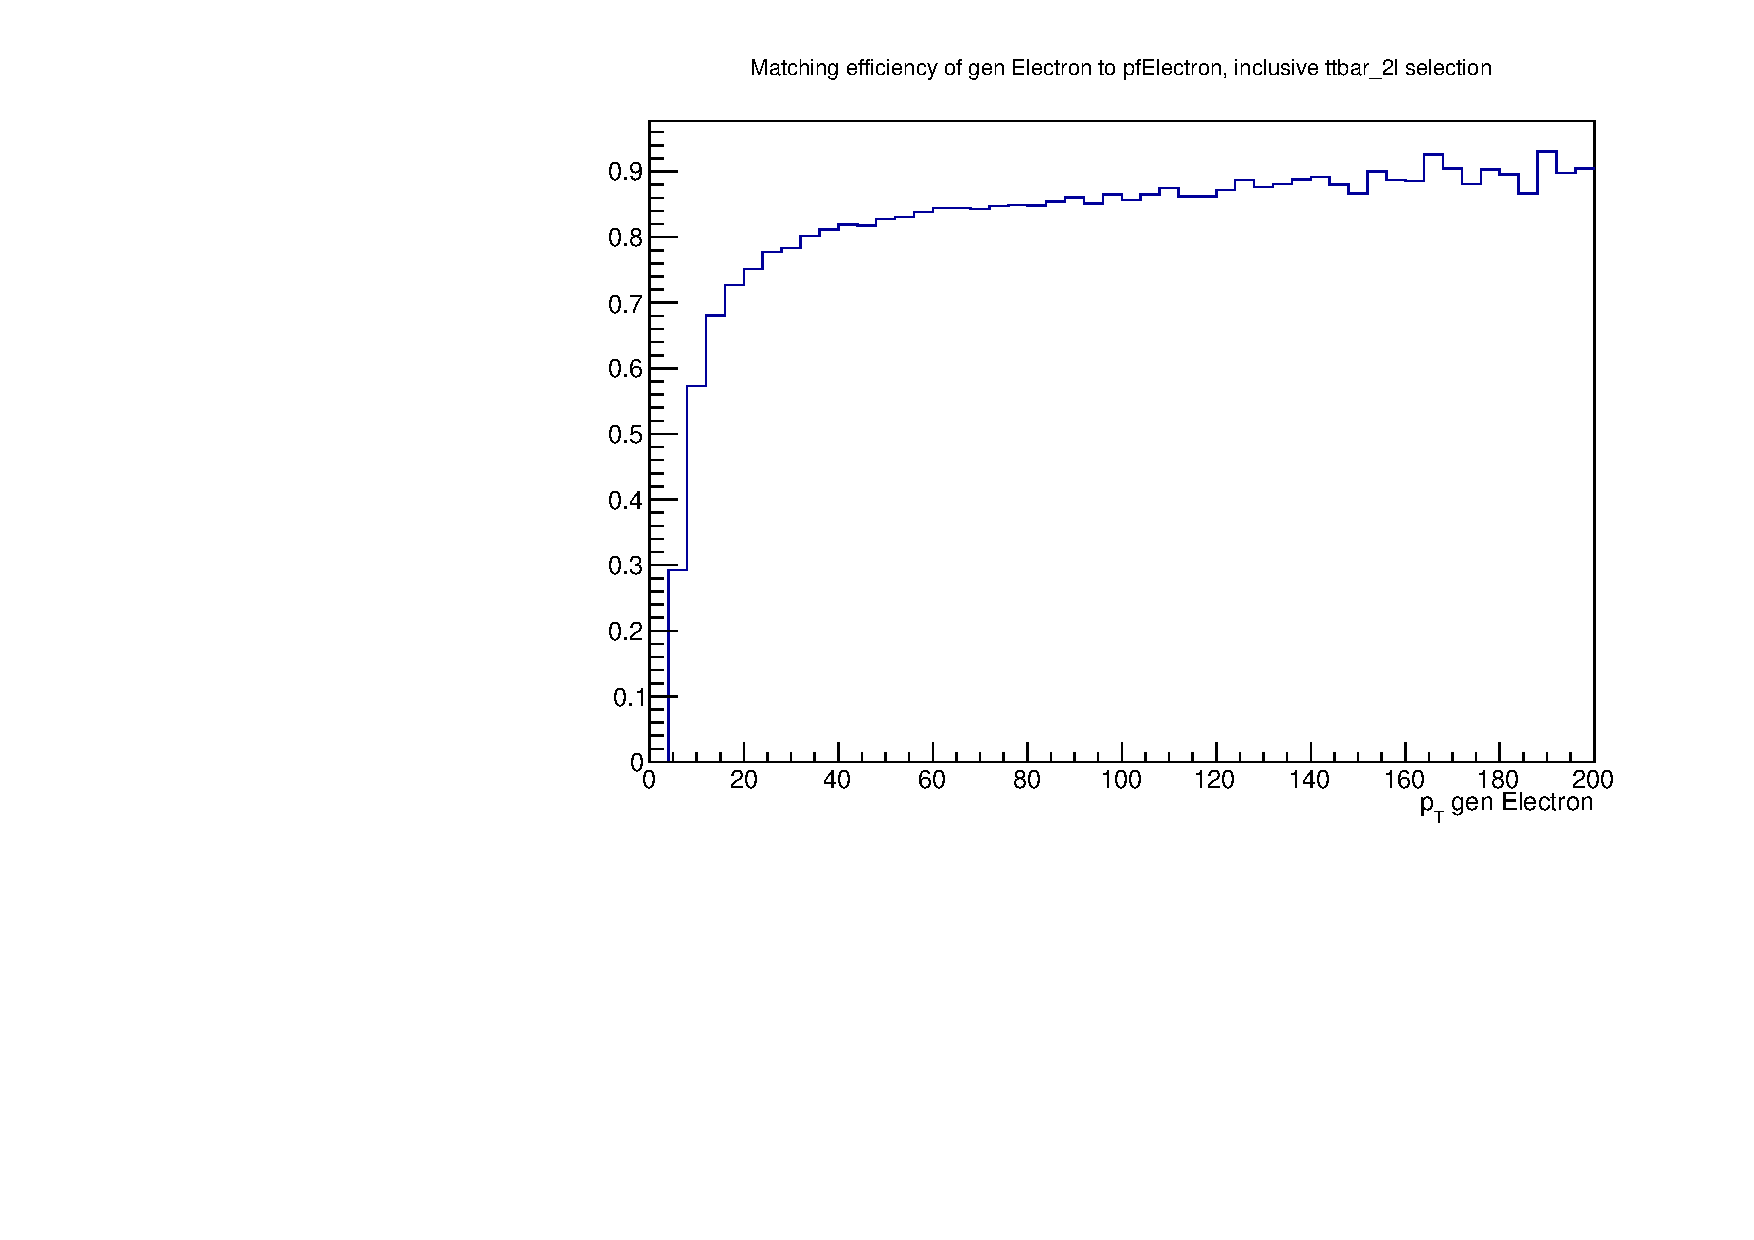
\includegraphics[width=0.60\textwidth]{Figures/studiesLostLepton/matchEff_genEl_to_pfEl_incl.pdf}
\caption{\label{fig:lost_lepton_studies:el_gen_matching_eff} Matching effiency vs $p_{T}$ between gen electrons and pfElectron candidates. }
\end{figure}

Approximately half of the lost leptons that pass the analysis selection are hadronically decaying taus, as shown in figure \ref{fig:lost_lepton_studies:classification}.  Of this 50\%, approximately 70\% of the hadronic tau decays are 1-prong, with the remaining approximately 30\% come from 3-prong decays.  Out of the lost electrons and muons, 8\% and 9\% of total lost leptons come from taus decaying to muons and leptons respectively.  Direct lost electrons compose approximately 17.5\% of the background, while director muons contribute approximately 14\%.  Since the leptons coming from tau decays will be softer in $p_{T}$ when compared to their direct counterparts, these will often fall out of acceptance and will difficult to tune cuts further in order to reject these events.  The largest impact in the analysis will come from reducing the 1-prong hadronically decaying taus.  Since these decays, by definition, will have a single isolated track, the use of tracker-baed isolation will be the best kinematic handle on reducing this background.  Since direct lepton decays also tend to be isolated, tracker isolation will also be used to target this background.  The 3-prong hadronic tau decays will be targeted using the MVA id.  

\begin{figure}[ht]
\centering
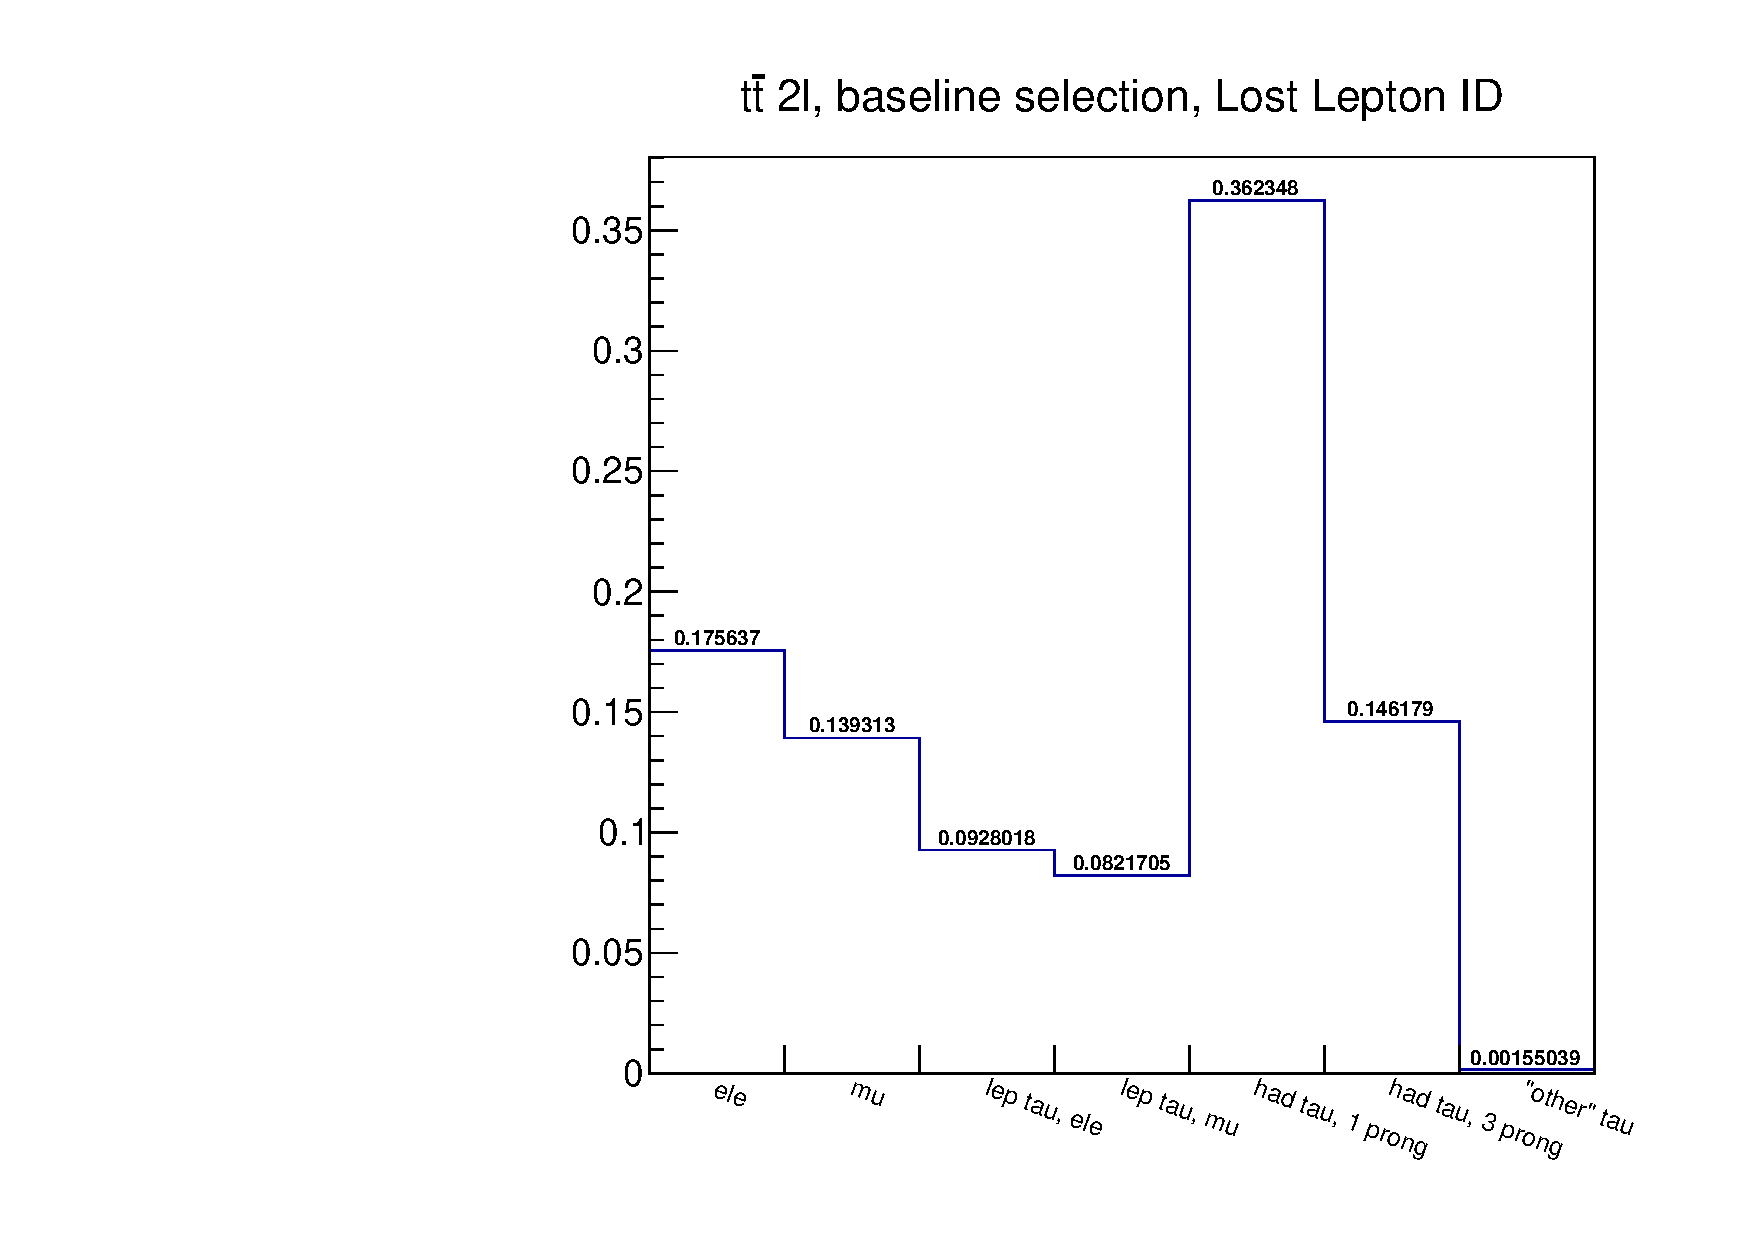
\includegraphics[width=0.60\textwidth]{Figures/studiesLostLepton/lostLeptonStudies__ttbar2l__lostLeptonID.pdf}
\caption{\label{fig:lost_lepton_studies:classification} Classification of the lost lepton flavour passing analysis selection }
\end{figure}

Next, it is important to understand the acceptance of these lost lepton events.  The majority of electron events, that fail acceptance, are from low pT.  Figure \ref{fig:lost_lepton_studies:el_acceptance} shows the $p_{T}$ and $\eta$ distrubtions for the lost gen electrons, including those coming from leptonic tau decays. Approximately 57\% of lost gen electrons pass the $p_{T}>5$GeV and $\eta<2.4$ cuts for the acceptance.    

\begin{figure}[ht]
\centering
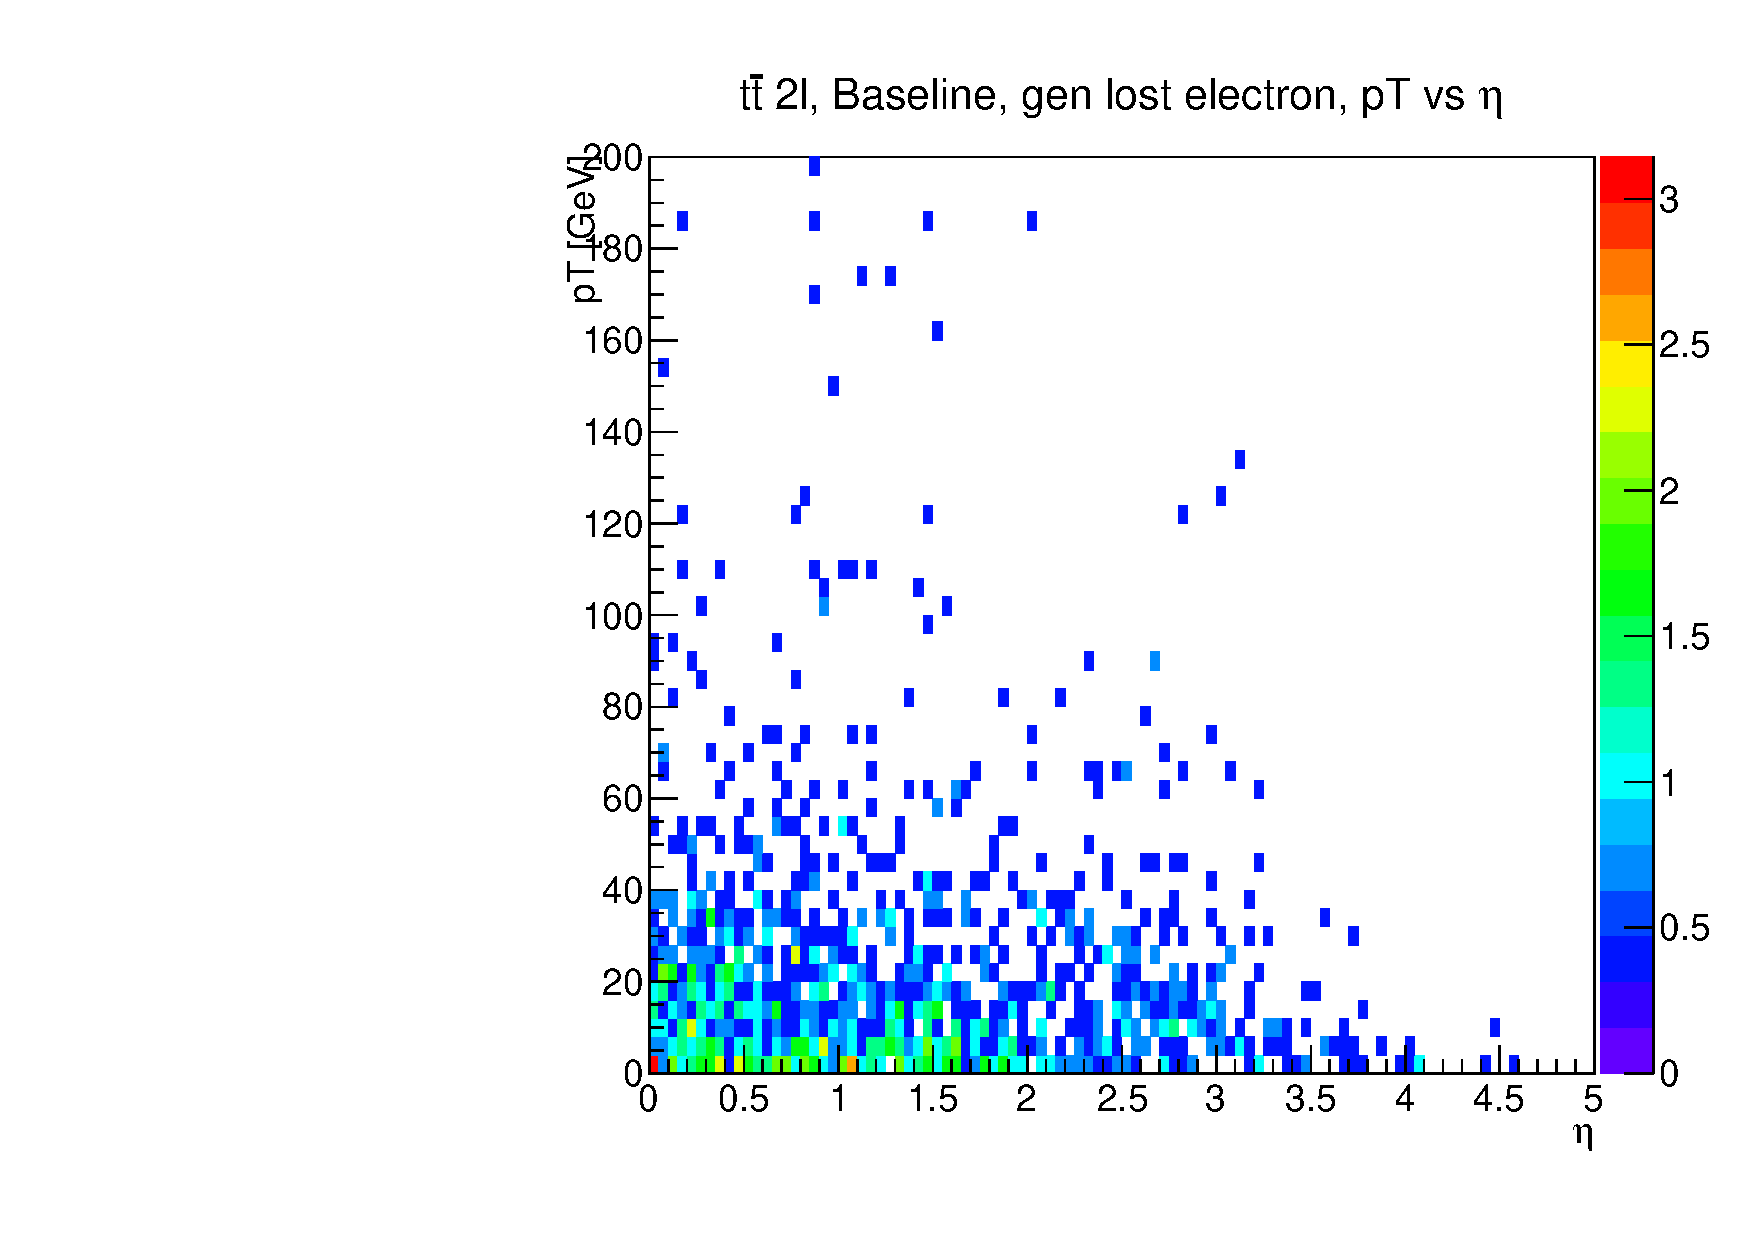
\includegraphics[width=0.32\textwidth]{Figures/studiesLostLepton/lostLeptonStudies__ttbar2l__genLostElectron__pt_vs_eta.pdf}
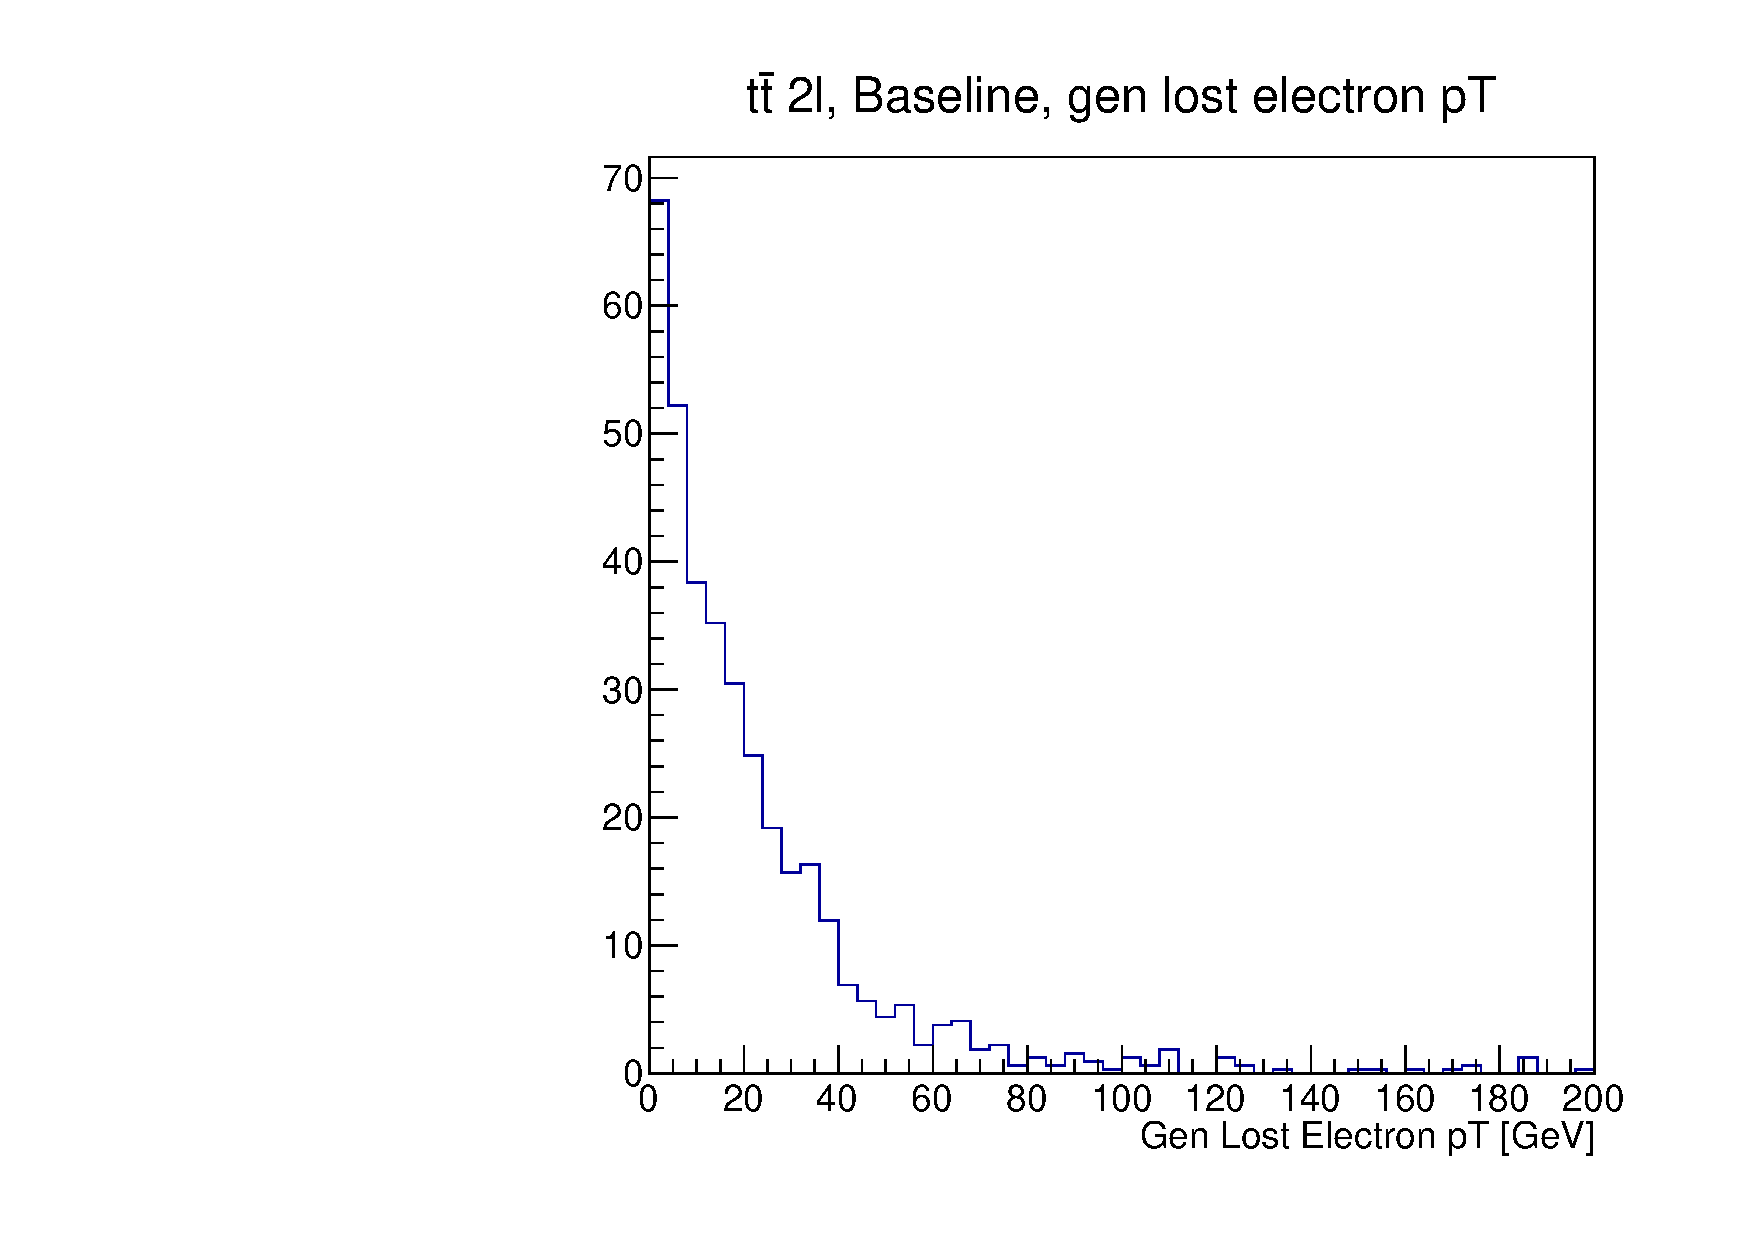
\includegraphics[width=0.32\textwidth]{Figures/studiesLostLepton/lostLeptonStudies__ttbar2l__genLostElectron__pt_vs_eta__projectionY__pt.pdf}
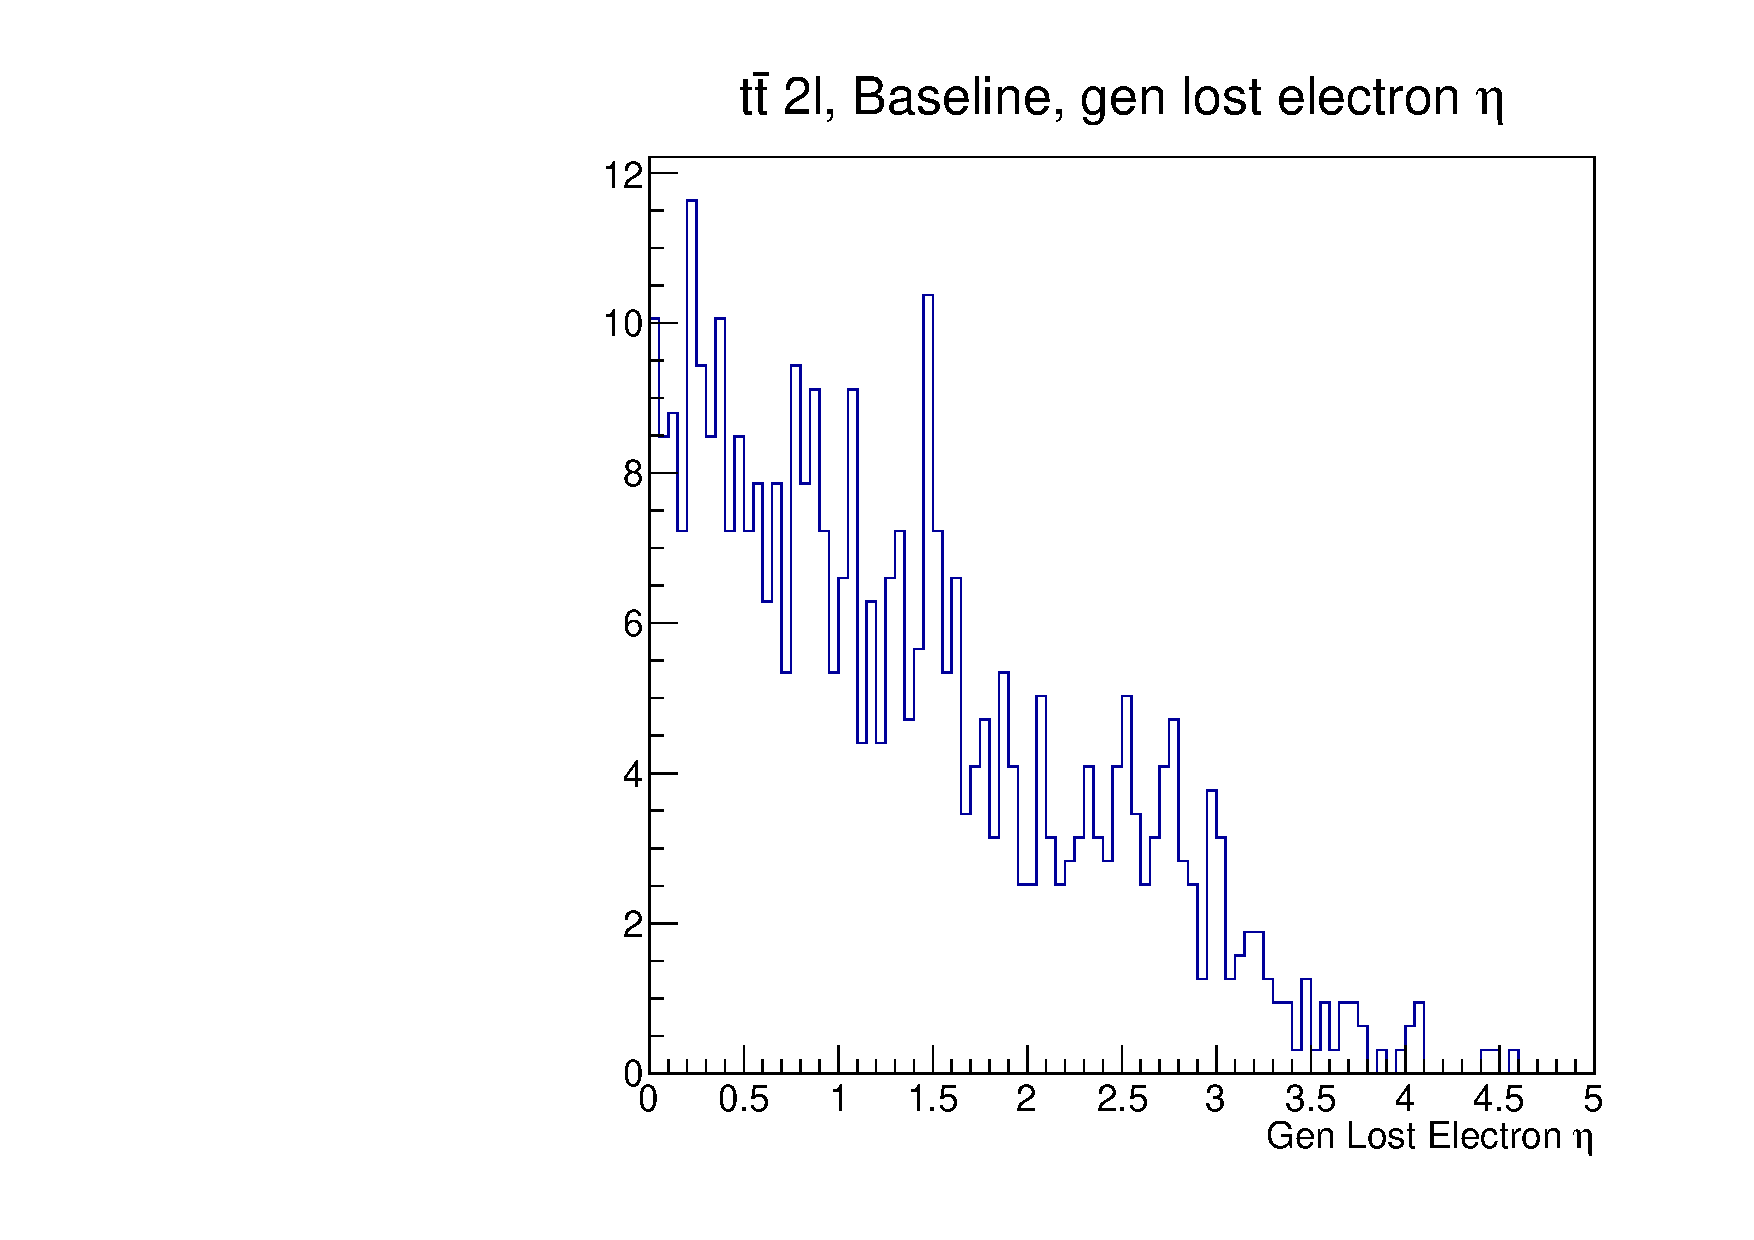
\includegraphics[width=0.32\textwidth]{Figures/studiesLostLepton/lostLeptonStudies__ttbar2l__genLostElectron__pt_vs_eta__projectionX__eta.pdf}
\caption{\label{fig:lost_lepton_studies:el_acceptance} (Left) Lost gen electron $p_{T}$ vs $\eta$, (Center) Projection from left-most plot, lost gen electron $p_{T}$ distribution, (Right) Projeciton from left-most plot, lost gen electron $\eta$ distribution.  Overall, only approximately 57\% of gen lost electrons pass acceptance }
\end{figure}

For muons, there are similar distributions in $p_{t}$ and $\eta$, for the lost gen muon.  While most events fail the $p_{T}>5$GeV cut, there are relatively more events, compared to gen lost electrons, that fail the $\eta<2.4$ acceptance cut.  


\subsection{Optimization of 8 TeV Lost Lepton Vetos for 13 TeV}
\label{sec:lost_lepton_studies:optimization}

